\chapter{Fachliche Grundlagen}
\label{cha:Fachliche Grundlagen}

Dieses Kapitel führt die theoretischen Grundlagen ein, auf denen das in dieser Arbeit entwickelte System aufbaut. Abschnitt~\ref{sec:reinforcement_learning} behandelt Reinforcement Learning als Lernparadigma und formalisiert das Problem als Markov Decision Process. Abschnitt~\ref{sec:ppo} stellt Lösungsverfahren vor, ausgehend von tabellarischen Methoden über Funktionsapproximation bis hin zu Proximal Policy Optimization, dem in dieser Arbeit eingesetzten Trainingsalgorithmus. Abschnitt~\ref{sec:cnn} beschreibt Convolutional Neural Networks als Architektur zur Verarbeitung räumlicher Sensordaten. Abschnitt~\ref{sec:aabb} definiert achsenparallele Begrenzungsboxen, die in dieser Arbeit zur Kollisionserkennung verwendet werden.

\section{Reinforcement Learning}
\label{sec:reinforcement_learning}

Reinforcement Learning bezeichnet das Lernen aus Interaktionen mit einer Umgebung, um ein Ziel zu erreichen. Ein Agent wählt in aufeinanderfolgenden Situationen Aktionen und erhält dafür numerische Belohnungen. Aus diesen Erfahrungen muss er eigenständig ableiten, welche Aktionen nicht nur unmittelbar, sondern auch langfristig den höchsten Ertrag erzielen. Sofern nicht anders angegeben, folgt die Darstellung in diesem Abschnitt \textcite{suttonReinforcementLearningIntroduction2020}.

\subsection{Markov Decision Process}
\label{subsec:mdp}
Ein \Fachbegriff{Markov Decision Process} (MDP) ist ein Modell, mit dem Reinforcement Learning Probleme präzise formalisiert werden können. Der Lerner und Entscheider wird als \NeuerBegriff{Agent} bezeichnet; alles außerhalb, womit der Agent interagiert und was er nicht willkürlich verändern kann, bildet die \NeuerBegriff{Umgebung}.

Die Interaktion zwischen Agent und Umgebung erfolgt in diskreten Zeitschritten $t = 0, 1, 2, \dots$. In jedem Schritt beobachtet der Agent einen \NeuerBegriff{Zustand} $S_t \in \mathcal{S}$, wählt auf dessen Grundlage eine \NeuerBegriff{Aktion} $A_t \in \mathcal{A}$ und erhält einen Zeitschritt später eine numerische \NeuerBegriff{Belohnung} $R_{t+1} \in \mathcal{R}$ sowie einen neuen Zustand $S_{t+1}$ (Abbildung~\ref{fig:mdp_agent_environment}).

\begin{figure}[H]
    \centering
    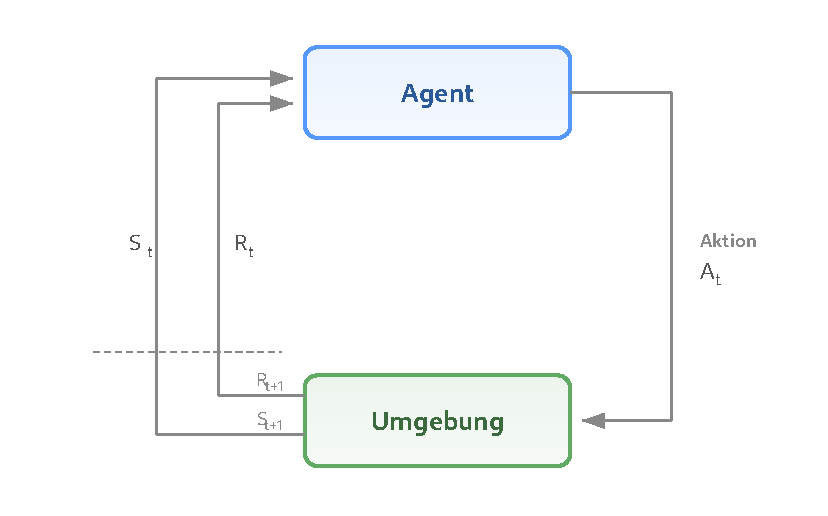
\includegraphics[width=0.65\linewidth]{Bilder/mdp_agent_environment.pdf}
    \caption{Interaktion zwischen Agent und Umgebung in einem MDP (nach \cite{suttonReinforcementLearningIntroduction2020}, S.~48).}
    \label{fig:mdp_agent_environment}
\end{figure}

Die Übergangsdynamik der Umgebung wird durch die Funktion
\begin{equation} \label{eq:mdp_dynamics}
    p(s', r \mid s, a) = \Pr\{S_{t+1} = s',\, R_{t+1} = r \mid S_t = s, A_t = a\}
\end{equation}
vollständig charakterisiert, welche die Wahrscheinlichkeit angibt, ausgehend vom Zustand $s$ bei gewählter Aktion $a$ in den Folgezustand $s'$ überzugehen und dabei die Belohnung $r$ zu erhalten. Wesentlich ist dabei die \Fachbegriff{Markov-Eigenschaft}: Folgezustand und Belohnung hängen ausschließlich vom gegenwärtigen Zustand-Aktions-Paar $(s,a)$ ab.

Das Ziel des Agenten besteht darin, durch Interaktion mit der Umgebung eine Strategie $\pi(a \mid s)$ zu identifizieren, welche die über die Zeit kumulierte Belohnung maximiert. Eine solche Strategie wird als \NeuerBegriff{optimale Strategie} bezeichnet und mit $\pi_*$ gekennzeichnet.



\section{Lösungen von MDPs}
\label{sec:ppo}

Welche Verfahren zur Bestimmung einer optimalen Strategie geeignet sind, hängt maßgeblich von der Formulierung des Reinforcement-Learning-Problems ab. Die klassische Theorie liefert exakte Lösungen ausschließlich für endliche MDPs mit vollständig bekanntem Übergangsmodell; ihre Grundideen lassen sich jedoch auf komplexere Problemklassen verallgemeinern.
Dieser Abschnitt behandelt die Lösung von MDPs. Eingeführt werden zunächst tabellarische Verfahren, anschließend Funktionsapproximation und schließlich Policy-Gradient-Methoden, die in das Verfahren der \Fachbegriff{Proximal Policy Optimization} (PPO) münden.

\subsection{Dynamische Programmierung}
\label{subsec:dp}

Das Ziel des Agenten besteht in der Maximierung des erwarteten Ertrags $G_t = \sum_{k=0}^{\infty} \gamma^k R_{t+k+1}$ mit Diskontierungsfaktor $\gamma \in [0,1)$. Die Güte einer Strategie $\pi$ wird durch die Zustandswertfunktion $v_\pi(s) = \mathbb{E}_\pi[G_t \mid S_t = s]$ charakterisiert, die den erwarteten Ertrag ausgehend von einem Zustand angibt. Die Zustandswertfunktion der optimalen Strategie $\pi_*$ wird als $v_*$ bezeichnet. Ihre direkte Berechnung setzt jedoch ein vollständig bekanntes Übergangsmodell und einen abzählbaren Zustandsraum voraus. In der Praxis sind beide Voraussetzungen selten gleichzeitig erfüllt: Das Übergangsmodell physikalischer Systeme ist in der Regel nicht vollständig bekannt, und selbst bei bekanntem Modell übersteigt der Zustandsraum realistischer Probleme typischerweise jene Dimensionen, in denen eine exakte Lösung mit vertretbarem Rechenaufwand möglich wäre.

\subsection{Monte-Carlo- und Temporal-Difference-Verfahren}
\label{subsec:mc_td}

Das fehlende Modell als erste Einschränkung wird durch \Fachbegriff{sample-basierte} Verfahren wie Monte-Carlo- und Temporal-Difference-Methoden (TD) aufgehoben. Monte-Carlo-Methoden benötigen den vollständigen Episodenertrag $G_t$ und können die Wertschätzung daher erst nach Abschluss einer Episode aktualisieren. TD-Verfahren hingegen nutzen \Fachbegriff{Bootstrapping} und korrigieren ihre Schätzung nach jedem einzelnen Zeitschritt anhand der geschätzten Bewertung des Folgezustands:
\begin{equation} \label{eq:td_update}
    V(S_t) \leftarrow V(S_t) + \alpha \bigl[R_{t+1} + \gamma\, V(S_{t+1}) - V(S_t)\bigr].
\end{equation}
TD-Verfahren bilden die Grundlage der meisten modernen Reinforcement-Learning-Algorithmen: Sie können online angewandt werden, benötigen wenig Rechenaufwand und lassen sich mit Funktionsapproximation auf große Zustandsräume skalieren.

\subsection{Funktionsapproximation}
\label{subsec:function_approximation}


Die Dimensionalität des Zustandsraums als zweite Einschränkung kann durch \NeuerBegriff{Funktionsapproximation} überwunden werden. Statt jeden Zustand mit einem eigenen Eintrag zu versehen, wird die Wertfunktion durch eine parametrisierte Funktion $\hat{v}(s, \mathbf{w})$ mit $\mathbf{w} \in \mathbb{R}^d$ und $d \ll |\mathcal{S}|$ dargestellt und in Richtung~$v_\pi$ optimiert.
Parametrisierte Funktionen erlauben Generalisierung: Erfahrungen, die über einen Zustand gemacht wurden, lassen sich auf benachbarte Zustände übertragen; gleichzeitig werden kontinuierliche Zustandsräume handhabbar. Als Parametrisierung eignen sich insbesondere neuronale Netze, da diese als universelle Funktionsapproximatoren in der Lage sind, beliebige stetige Funktionen auf kompakten Teilmengen beliebig genau anzunähern \autocite{hornikMultilayerFeedforwardNetworks1989}.

Während die Funktionsapproximation das Problem kontinuierlicher Zustandsräume löst, bleibt ein zweites Hindernis bei kontinuierlichen \emph{Aktionsräumen} bestehen. Wertbasierte Verfahren wählen Aktionen gemäß $a = \arg\max_{a'} \hat{q}(s, a', \mathbf{w})$; dieses Maximum ist in kontinuierlichen Aktionsräumen jedoch im Allgemeinen nicht effizient berechenbar.

\subsection{Policy-Gradient-Methoden}
\label{subsec:policy_gradient}

Eine Alternative ist, die Strategie nicht über eine Wert-Funktion abzuleiten, sondern direkt als parametrisierte Funktion $\pi(a \mid s, \boldsymbol{\theta})$ zu beschreiben und ihre Parameter $\boldsymbol{\theta}$ durch Gradientenaufstieg zu optimieren. Der entscheidende Vorteil für diese Arbeit: Policy-Gradient-Methoden können auf natürliche Weise kontinuierliche Aktionsräume handhaben, wie sie in der Drohnensteuerung auftreten.

In der Praxis wird der Policy-Gradient-Ansatz häufig als \Fachbegriff{Actor-Critic-Architektur} umgesetzt: Ein \Fachbegriff{Actor}-Netz repräsentiert die Strategie $\pi(\cdot \mid \cdot, \boldsymbol{\theta})$, ein \Fachbegriff{Critic}-Netz schätzt eine Wert-Funktion $\hat v(\cdot, \mathbf{w})$. Die Wertschätzung des Critics dient als Referenzniveau, das die Varianz der Gradientenschätzung reduziert, ohne sie zu verzerren.

\subsection{Proximal Policy Optimization}
\label{subsec:ppo_clip}

Eine moderne und in der Praxis weit verbreitete Variante des Policy-Gradient-Ansatzes ist \Fachbegriff{Proximal Policy Optimization} (PPO) \autocite{schulmanProximalPolicyOptimization2017}, ein Actor-Critic-Verfahren, das die Trainingsstabilität von Trust-Region-Methoden erreicht und dabei wesentlich einfacher zu implementieren ist.

Zu große Strategieänderungen pro Optimierungsschritt können Policy-Gradient-Verfahren
destabilisieren, da die gesammelten Trajektorien für die veränderte Strategie nicht mehr
repräsentativ sind \autocite{schulmanProximalPolicyOptimization2017}. Trust-Region-Methoden
wie TRPO \autocite{schulmanTrustRegionPolicy2015} begrenzen daher die KL-Divergenz
zwischen aufeinanderfolgenden Strategien, erfordern dafür jedoch Approximationen zweiter
Ordnung. PPO erzielt eine vergleichbare Stabilisierung allein durch eine geklippte
Zielfunktion:
\begin{equation} \label{eq:ppo_clip}
    L^{\mathrm{CLIP}}(\boldsymbol{\theta}) = \hat{\mathbb{E}}_t\!\left[
        \min\!\left(
            r_t(\boldsymbol{\theta})\,\hat{A}_t,\;
            \mathrm{clip}\!\left(r_t(\boldsymbol{\theta}),\, 1-\varepsilon,\,
            1+\varepsilon\right) \hat{A}_t
        \right)
    \right],
\end{equation}
wobei $r_t(\boldsymbol{\theta}) = \pi_{\boldsymbol{\theta}}(a_t \mid s_t)\,/\,
\pi_{\boldsymbol{\theta}_{\mathrm{alt}}}(a_t \mid s_t)$ das
Wahrscheinlichkeitsverhältnis zwischen neuer und alter Strategie ist, $\hat{A}_t$ der
Vorteilsschätzer und $\varepsilon$ die Clipping-Grenze.
Das Clipping bewirkt \emph{pessimistische} Updates: Verbessert eine Strategieänderung
das Objective, wird der Anreiz bei $r_t > 1 + \varepsilon$ gekappt; verschlechtert sie
es, greift die Minimumbildung und die Korrektur bleibt uneingeschränkt
(Abbildung~\ref{fig:ppo_clip}). So werden zu große Schritte in Richtung guter
Erfahrungen gebremst, während schlechte Aktionen voll korrigiert werden.

\begin{figure}[ht]
    \centering
    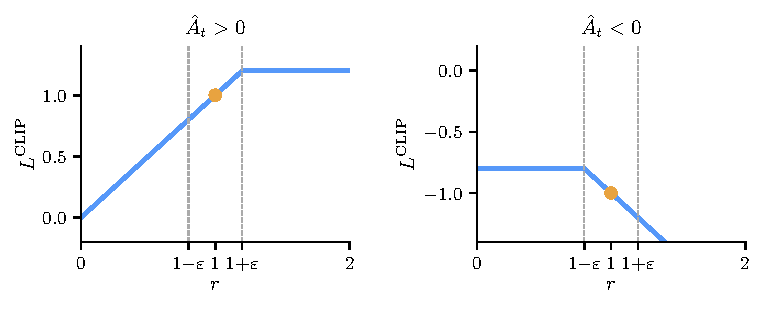
\includegraphics[width=0.85\linewidth]{Bilder/ppo_clipping.pdf}
    \caption{$L^{\mathrm{CLIP}}$ als Funktion des
    Wahrscheinlichkeitsverhältnisses~$r$. Links ($\hat{A}_t > 0$): der Anreiz wird bei
    $1 + \varepsilon$ gekappt. Rechts ($\hat{A}_t < 0$): die Korrektur bleibt
    uneingeschränkt (nach \autocite{schulmanProximalPolicyOptimization2017}, Fig.~1).}
    \label{fig:ppo_clip}
\end{figure}

Das vollständige PPO-Objective kombiniert das Clipping mit zwei weiteren Termen:
\begin{equation} \label{eq:ppo_full}
    L(\boldsymbol{\theta}) =
    L^{\mathrm{CLIP}}(\boldsymbol{\theta})
    - c_1\, L^{VF}(\boldsymbol{\theta})
    + c_2\, H\!\left[\pi_{\boldsymbol{\theta}}\right]\!(s_t),
\end{equation}
wobei $L^{VF} = (V_{\boldsymbol{\theta}}(s_t) - V_t^{\mathrm{targ}})^2$ der quadratische
Fehler der Wertfunktionsschätzung des Critics ist und
$H[\pi_{\boldsymbol{\theta}}]$ einen Entropie-Bonus bezeichnet, der vorzeitige
Konvergenz der Aktionsverteilung verhindert. Ohne diesen Term kann die
Standardabweichung gegen null konvergieren (\Fachbegriff{Std-Collapse}), was die Strategie
irreversibel auf eine deterministische Aktion festlegt.

Für die Schätzung des Vorteils~$\hat{A}_t$ wird \Fachbegriff{Generalized Advantage Estimation}
(GAE) \autocite{schulmanHighDimensionalContinuousControl2016} eingesetzt, das über den
Parameter~$\lambda$ einen Kompromiss zwischen Bias und Varianz der Vorteilsschätzung
steuert.

\section{Convolutional Neural Networks}
\label{sec:cnn}

\NeuerBegriff{Convolutional Neural Networks} (CNNs) sind eine Klasse neuronaler Netze, die speziell für die Verarbeitung von Daten mit räumlicher Struktur entwickelt wurden, etwa Bilder in Form zweidimensionaler Pixelarrays. Sofern nicht anders angegeben, folgt die Darstellung in diesem Abschnitt \textcite{lecunDeepLearning2015}.

Die Architektur eines CNN besteht aus einer Kaskade von Faltungs- und Pooling-Schichten. In einer \Fachbegriff{Faltungsschicht} sind die Einheiten in sogenannten \Fachbegriff{Feature Maps} organisiert. Jede Einheit ist nur mit einem lokalen Ausschnitt der vorherigen Schicht verbunden und verrechnet diesen mit einem \Fachbegriff{Filter} (auch \Fachbegriff{Kernel}), einer kleinen quadratischen Gewichtsmatrix \autocite{botschParametrischeMethoden2023}. Dabei werden die überdeckten Eingabewerte elementweise mit den Filtergewichten multipliziert und zu einem einzelnen Ausgabewert aufsummiert. Alle Einheiten innerhalb einer Feature Map teilen denselben Filter; mathematisch entspricht diese Operation einer diskreten Faltung. Verschiedene Feature Maps innerhalb einer Schicht verwenden unterschiedliche Filter und erkennen dadurch unterschiedliche lokale Muster. Die Filtergewichte werden nicht manuell festgelegt, sondern während des Trainings gelernt \autocite{botschParametrischeMethoden2023}. Die gemeinsame Nutzung der Gewichte beruht auf zwei Eigenschaften natürlicher Bilddaten: Benachbarte Werte bilden häufig korrelierte lokale Muster, und diese Muster treten unabhängig von ihrer Position im Bild auf.

\Fachbegriff{Pooling-Schichten} fassen die Aktivierungen benachbarter Einheiten zusammen, typischerweise durch Auswahl des Maximums innerhalb eines lokalen Fensters (\Fachbegriff{Max-Pooling}) \autocite{botschParametrischeMethoden2023}. Dies reduziert die räumliche Auflösung der Repräsentation und erzeugt eine gewisse Invarianz gegenüber kleinen Verschiebungen im Eingabebild.

Durch das Stapeln mehrerer Faltungs- und Pooling-Stufen entsteht eine hierarchische Merkmalsextraktion: Frühe Schichten erkennen einfache lokale Strukturen wie Kanten, mittlere Schichten kombinieren diese zu komplexeren Motiven, und tiefe Schichten repräsentieren ganze Objektteile. Die resultierende kompakte Repräsentation kann als Eingabe für nachgeschaltete Netzwerkkomponenten dienen. \textcite{mnihHumanlevelControlDeep2015} zeigten erstmals, dass ein CNN in dieser Rolle als Merkmalsextraktor innerhalb eines Reinforcement-Learning-Systems eingesetzt werden kann, indem sie eine Strategie direkt aus hochdimensionalen Bilddaten lernten.

\section{Achsenparallele Begrenzungsboxen}
\label{sec:aabb}

Eine \NeuerBegriff{achsenparallele Begrenzungsbox} (\Fachbegriff{Axis-Aligned Bounding Box}, AABB) ist das kleinste achsenparallele Quader, das ein gegebenes Objekt vollständig umschließt. Sie wird durch zwei Punkte definiert: das komponentenweise Minimum und Maximum aller Objektpunkte,
\begin{equation}
    \mathbf{p}_{\min} = \bigl(\min_i x_i,\, \min_i y_i,\, \min_i z_i\bigr), \quad
    \mathbf{p}_{\max} = \bigl(\max_i x_i,\, \max_i y_i,\, \max_i z_i\bigr),
\end{equation}
wobei $(x_i, y_i, z_i)$ die Eckpunkte bzw.\ Oberflächenpunkte des Objekts bezeichnen.

Die AABB besitzt eine \Fachbegriff{konservative} Eigenschaft: Da sie das Objekt vollständig umschließt, wird jede tatsächliche Kollision mit dem Objekt auch als Kollision mit der AABB erkannt. Im Umkehrschluss kann ein Punkt jedoch innerhalb der AABB liegen, ohne das eingeschlossene Objekt zu berühren. Der Approximationsfehler wächst mit der Abweichung der Objektgeometrie von einer quaderförmigen Gestalt; bei konkaven oder stark unregelmäßigen Formen kann die AABB ein erheblich größeres Volumen als das Objekt selbst einnehmen.

Für die Kollisionserkennung in Echtzeitsystemen bietet die AABB einen günstigen Kompromiss: Der Abstandstest reduziert sich auf sechs skalare Vergleiche pro Achse und ist damit wesentlich effizienter als Distanzberechnungen auf der tatsächlichen Objektgeometrie. Dem steht die beschriebene konservative Approximation gegenüber, die zu falsch-positiven Kollisionserkennungen führen kann.